\section{Arrays and vectors}
\begin{itemize}
    \item Arrays and vectors are compound data types. Which means they are data types made out of other data types.
\end{itemize}

\section{What is an array?}
\begin{itemize}
    \item An array is a compound data type or a data structure.
        \begin{itemize}
            \item Which means they are data types composed of other data types. They allow us to have collections of elements. 
        \end{itemize}
    \item All elements are of the same type.
    \item Each element can be accessed directly.
    \item Why do we need arrays?
        \begin{itemize}
            \item Suppose we would need to store the scores of a test. 
            \item We could declare $n$ variables for $n$ students:
                \begin{minted}[autogobble]{cpp}
                    int test_score_1 {0};
                    int test_score_2 {0};
                    int test_score_3 {0};
                    int test_score_4 {0};
                    // ...
                    int test_score_100 {0};
                \end{minted}
            
            \item This becomes tedious and error prone, now you would need to keep track of 100 variables with their own name. And even worse if I have 1,000,000 test scores this would get out of hand very easily.
            \item In this case it's better to use an array.
        \end{itemize}
\end{itemize}

\subsection{Characteristics}
\begin{itemize}
    \item Fixed size. 
    \item Elements are all the same type.
    \item Stored contigously in memory.
    \item Individual elements can be accessed by their position or index.
    \item First element is at index 0.
    \item Last element is at index $size-1$.
    \item No checking to see if you are out of bounds. It is the responsability of the programmer to check if the program is writing data out of bounds, this can cause undefined behaviour.
    \item Always initialize arrays.
    \item Very efficient.
    \item Iteration (looping) is often used to process the elements stored.
\end{itemize}
\begin{figure}[H]
    \centering
    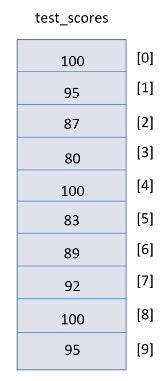
\includegraphics[width=0.4\textwidth]{./figs/arrays.png}
\end{figure}


%----------------------------------------------------------------------------------------
\section{Declaring and initializing arrays}
\subsection{Declaring arrays}
\begin{itemize}
    \item \verb|element_type array_name [constant number of elements];|
        \begin{itemize}
            \item The constant number of elements can be an expression that evaluates to a constant, a constant, a number or anything that results in a number before compiling.
        \end{itemize}
        \begin{minted}[autogobble]{cpp}
            int test_scores[5];
            int high_score_per_level[10];
            const double days_in_year {365};
            double hi_temperature[days_in_year];
        \end{minted}
\end{itemize}

\subsection{Initializing arrays}
\begin{itemize}
    \item \verb|element_type array_name [number of elements] {init elements}; |
        \begin{minted}[autogobble]{cpp}
            int test_scores[5] {100,95,99,87,88};
            int high_score_per_level[10] {3,5}; // init to 3,5 and remaining to 0.
            const double days_in_year {365}; 
            double hi_temperatures[days_in_year] {0}; // init all to zero.
            double hi_temperature[days_in_year] {1,2,3,4,5}; // size automatically calculated.
        \end{minted}
\end{itemize}



%----------------------------------------------------------------------------------------
\section{Accessing and modifying array elements}
\begin{itemize}
    \item Accessing array elements: \verb|array_name [element_index];|.
        \begin{minted}[autogobble]{cpp}
            #include <iostream>
            using namespace std;
            int main() {
                int test_scores[5] {100,95,99,87,88};
                cout << "index 0: " << test_scores[0] << endl;
                cout << "index 1: " << test_scores[1] << endl;
                cout << "index 2: " << test_scores[2] << endl;
                cout << "index 3: " << test_scores[3] << endl;
                cout << "index 4: " << test_scores[4] << endl;
                return 0;
            } 
            /* OUTPUT: 
            index 0: 100
            index 1: 95
            index 2: 99
            index 3: 87
            index 4: 88
            */
        \end{minted}
    
    \item Changing contents of array elements: 
        \begin{minted}[autogobble]{cpp}
            #include <iostream>
            using namespace std;
            int main() {
                int test_scores[5] {0};
                cin >> test_scores[0];
                cin >> test_scores[1];
                cin >> test_scores[2];
                cin >> test_scores[3];
                cin >> test_scores[4];
                test_scores[0] = 90;
                return 0;
            } 
        \end{minted}
\end{itemize}

\subsection{How do arrays work?}
\begin{itemize}
    \item The nane of the array represents the location of the first element in the array (index 0).
    \item The [index] represents the offset from the beggining of the array.
    \item C++ simply performs a calculation to find the correct element.
    \item There is no bounds checking.
\end{itemize}

\subsection{Examples}
\begin{minted}[autogobble]{cpp}
    #include <iostream>
    using namespace std;
    int main() {
        char vowels[] {'a','e','i','o','u'};
        cout << vowels[0] << endl; 
        cout << vowels[4] << endl; 
        cin >> vowels[5]; // out of bounds.
        return 0;
    }
    /* OUTPUT:
        a
        u
        ... program crashes.
    */
\end{minted}
\begin{minted}[autogobble]{cpp}
    #include <iostream>
    using namespace std;
    int main() {
        double hi_temps[] {90.1, 89.8, 77.5, 81.6};
        cout << "\nThe fist high temperature is: " << hi_temps[0] << endl;
        hi_temps[0] = 100.7; // sets the first element of hi_temps to 100.7.
        cout << "\nThe fist is now: " << hi_temps[0] << endl;
        return 0;
    } 
    /* OUTPUT: 

    The fist high temperature is: 90.1

    The fist is now: 100.7

    */
\end{minted}

\begin{minted}[autogobble]{cpp}
    #include <iostream>
    using namespace std;
    int main() {
        int test_scores[5] {100};
        cout << "\nFirst score at index 0: " << test_scores[0] << endl;
        cout << "\nSecond score at index 1: " << test_scores[1] << endl;
        cout << "\nThird score at index 2: " << test_scores[2] << endl;
        cout << "\nFourth score at index 3: " << test_scores[3] << endl;
        cout << "\nFifth score at index 4: " << test_scores[4] << endl;
        cin >> test_scores[0];
        cin >> test_scores[1];
        cin >> test_scores[2];
        cin >> test_scores[3];
        cin >> test_scores[4];
        cout << "\nFirst score at index 0: " << test_scores[0] << endl;
        cout << "\nSecond score at index 1: " << test_scores[1] << endl;
        cout << "\nThird score at index 2: " << test_scores[2] << endl;
        cout << "\nFourth score at index 3: " << test_scores[3] << endl;
        cout << "\nFifth score at index 4: " << test_scores[4] << endl;
        return 0;
    } 
    /* OUTPUT:
    First score at index 0: 100

    Second score at index 1: 0

    Third score at index 2: 0

    Fourth score at index 3: 0

    Fifth score at index 4:  
    
    0 1 2 3 4 5

    First score at index 0: 1

    Second score at index 1: 2

    Third score at index 2: 3

    Fourth score at index 3: 4

    Fifth score at index 4: 5
    */
\end{minted}

\begin{minted}[autogobble]{cpp}
    #include <iostream>
    using namespace std;
    int main() {
        int test_scores[5] {100};
        cout << "Name of array: " << test_scores << endl;
        return 0;
    } 
    /* OUTPUT:
    Name of array: 0x61fe00
    */
\end{minted}


%----------------------------------------------------------------------------------------
\section{Multidimentional arrays}
\begin{itemize}
    \item Declaring multidimentional arrays: \verb|element_type array_name [dimension 1 size][dimension 2 size]...;|
        \begin{minted}[autogobble]{cpp}
            int movie_rating [3][4];
        \end{minted}
    
    \item Some compilers do place limits on the number of dimensions you have depending on what machine they are running and the compiler being used.
    \item Multi-dimentional arrays are a spreadsheet concept, think of the first dimension as the rows and the second as the columns.
\end{itemize}
\begin{minted}[autogobble]{cpp}
    int spread_sheet[][] {
        {1,2,3},
        {4,5,6},
        {7,8,9}
    };
\end{minted}


%----------------------------------------------------------------------------------------
\section{Declaring and initializing vectors}
\begin{itemize}
    \item Suppose we want to store test scores for my school.
    \item I have no way of knowing how many students will register next year.
    \item Options: 
        \begin{itemize}
            \item Pick a size that you are not likely to exceed and use static arrays.
            \item Use a dynamic array sich as a vector.
        \end{itemize}
\end{itemize}

\subsection{Vectors}
\begin{itemize}
    \item A C++ vector is a container in the C++ standard template library.
    \item An array that can grom and shrink in size at excecution time.
    \item Provides similar semantics and syntax as arrays.
    \item Very efficient.
    \item Can provide bounds checking.
    \item Can use lots of cool functions like sort, reverse, find and more.
    \item When we create a C++ vector we are creating a C++ object and this means it can perform operations for us.
\end{itemize}

\subsection{Declaring vectors}
\begin{itemize}
    \item We must include the vector library and the standard library, both allow us to create C++ vectors. 
    \item Syntax: \verb|vector<datatype> vector_name;|.
        \begin{minted}[autogobble]{cpp}
            #include <vector> 
            using namespace std;
            vector<char> vowels;
            vector<int> test_scores;
        \end{minted}
\end{itemize}

\subsection{Initializing vectors}
\begin{itemize}
    \item For vectors, since they are objects, we can provide initialization with the constructor intialization style: 
        \begin{minted}[autogobble]{cpp}
            vector<char> vowels (5);
            vector<int> test_scores (10);
        \end{minted}
        \begin{itemize}
            \item The above code creates a vector of size 5 if chars, then a vector of size 10 of ints, also all the elements of the array are intialized automatically to zero, you no longer need to do that explicitly.
        \end{itemize}
    
    \item We can also use the curly brace initialization style to specify the value of the elements we want:
        \begin{minted}[autogobble]{cpp}
            vector<char> vowels {'a','e','i','o','u'};
            // Initializes vowels to the specified values in a vector of size 5.
            vector<int> test_scores {100,98,89,85,93};
            // Initializes test_scores to the 5 specified values.
            vector<double> hi_temperatures (365, 80.0);
            // The first paramenter is the initial size of the vector which os 365, the second is to which value you want to initialize all the elements in the vector.
        \end{minted}
\end{itemize}

\subsection{Vector caracteristics}
\begin{itemize}
    \item Dynamic size. 
    \item Elements are all the same type.
    \item Stored contiguosly in memory.
    \item Individual elements can be accessed by their position or index.
    \item First element is at index 0.
    \item Last element is at index $size-1$.
    \item If you use the subscript operator ([index]) then vectors will provide no bounds checking, however the vector object allows you to get information at an index using methods that do provide bounds checking.
    \item Provides many useful functions that do bounds checking.
    \item Elements are automatically initialized to zero unless you specify otherwise.
    \item Very efficient.
    \item Iteration (looping) is ften used to process the elements.
\end{itemize}


%----------------------------------------------------------------------------------------
\section{Accessing and modifying vector elements}
\begin{itemize}
    \item The first way to access vector elements is to use array syntax (with the subscript operator): \verb|vector_name[element_index];| with this way no bounds checking will be done.
        \begin{minted}[autogobble]{cpp}
            vector<int> test_scores {100,95,99,87,88};
            cout << test_scores[0] << endl;
            cout << test_scores[1] << endl;
            cout << test_scores[2] << endl;
            cout << test_scores[3] << endl;
            cout << test_scores[4] << endl;
        \end{minted}
    \item We can also access vector elements with the \verb|.at| method, the syntax is: \verb|vector_name.at(element_index);|
        \begin{minted}[autogobble]{cpp}
            vector<int> test_scores {100,95,99,87,88};
            cout << test_scores.at(0) << endl;
            cout << test_scores.at(1) << endl;
            cout << test_scores.at(2) << endl;
            cout << test_scores.at(3) << endl;
            cout << test_scores.at(4) << endl;
        \end{minted}
\end{itemize}

\subsection{Vectors changing in size dynamically}
\begin{itemize}
    \item The vector has a method called \verb|push_back| that adds a new element (of the same type) to the back of the vector.
    \item This vector method will automatically allocate the required space.
\end{itemize}

\subsection{Out of bounds errors}
\begin{itemize}
    \item What if you are out of bounds?
    \item Arrays never do bounds checking.
    \item Many vector methods provide bounds checking.
    \item An exception and error message is generated.
\end{itemize}
